%!TEX root = ../../csuthesis_main.tex

\chapter{CORnet-S模型复现与基线分析}

\section{复现流程与实验配置}

CORnet-S模型是类脑视觉建模中典型的时间递归结构模型,其引入“时间步”(time steps)以模拟视觉皮层多次循环加工过程。为验证该模型在轻量级图像分类任务中的性能表现,并为后续结构改进提供对照基线,本文在Tiny-ImageNet-200数据集上对CORnet-S进行了完整复现与训练。

\subsection{数据集选型与预处理}

Tiny-ImageNet-200是ImageNet数据集的轻量级衍生版本,包含200个类别,每个类别下含有500张训练图像、50张验证图像和50张测试图像,图像均为RGB三通道,分辨率为64×64,数据集总规模约为120000张\cite{le2015tiny}。相比较于原始ImageNet(包含1000个类别,超过120万张图像),Tiny-ImageNet在保留多类别识别任务结构的同时大幅减少了数据规模,显著降低了模型调试、验证和分析的训练成本,特别适合用于轻量级模型测试与类脑结构优化实验以及在硬件需求不足的情况下使用。

\begin{table}[htb]
	\centering
	\caption{Tiny-ImageNet 数据集结构与规模统计表}
	\label{tab:tinyimagenet}
	\begin{tabular}{lllll}
		\hline
		数据划分 & 类别数 & 每类图像数 & 总图像数 & 图像尺寸 \\
		\hline
		训练集(train) & 200 & 500  & 100,000  & 64 × 64 × 3 \\
		验证集(val)   & 200 & 50   & 10,000   & 64 × 64 × 3 \\
		测试集(test)  & 200 & —    & 10,000   & 64 × 64 × 3 \\
		\textbf{合计}   & \textbf{200} & — & \textbf{120,000} & — \\
		\hline
	\end{tabular}
\end{table}

从数据内容以及结构上来看,Tiny-ImageNet覆盖了自然场景中的动物、植物、器具、交通工具等多种类别,图像采集来源广泛,标注准确,是一个兼具语义多样性与任务完整性的视觉识别基准数据集。由于其类别标签与ImageNet synset保持一致,该数据集也可用于ImageNet预训练模型的微调与迁移学习实验,具有良好的通用性和拓展性。Tiny-ImageNet使用了严格的目录层级组织方式。训练集以每类一个子文件夹的形式存储图像,验证集与测试集通过单独的索引文件(val\_annotations.txt)提供图像路径与标签对应关系,方便使用PyTorch等深度学习框架进行批量加载与处理。

在数据预处理过程中,训练集图像首先进行了随机裁剪与随机水平翻转的增强操作,以提升模型对尺度与姿态变化的泛化能力。考虑到后续模型结构设计参考了ImageNet预训练风格,输入尺寸统一调整为$224×224$,标准化处理均值为$[0.485,0.456,0.406]$,标准差为$[0.229,0.224,0.225]$。

验证集和测试集则使用统一的中心裁剪策略,并统一缩放到$224×224$,以保证评估过程的稳定性,避免因数据增强带来的评估波动,确保模型在不同实验间具有可比性。所有图像在进入模型前均经过ToTensor( )转换并执行标准化处理,保持与ImageNet预训练模型输入风格一致。

在数据加载实现上,本文使用PyTorch框架中的ImageFolder接口对训练集与验证集目录进行加载,并分别设置了4个并行数据读取线程(num\_workers=4),有效缓解数据读取瓶颈对GPU训练过程的影响,提高训练效率。


\subsection{模型加载与训练细节}

本文使用原始CORnet项目中公开的CORnet-S模型结构代码,并基于Kubilius等人在NeurIPS 2019论文中发布的配置进行参数设定\cite{kubilius2019brain}。CORnet-S模型遵循生物视觉皮层的区域划分设计,主要包含四个模块(V1、V2、V4、IT),分别对应灵长类视觉通路的层级区域。其中,V2、V4和IT模块均内置时间步递归机制,输入图像会在多个时间步内重复处理,使模型具备“类再入处理”的表征能力。各时间步之间共享卷积核参数,从而避免模型参数量过多的膨胀问题,增强时间建模的稳定性。

模型的decoder部分由全局平均池化层与全连接线性层组成,用于对IT模块的输出特征图进行压缩与分类映射。考虑到模型初始结构是为ImageNet原始任务设计,输出维度被设定为1000,对应ImageNet的1000个语义标签。在本研究中,虽然实际使用的是Tiny-ImageNet数据集(共200类),但为保持与原项目训练流程的一致性,结构仍保留1000维输出,但后续仅使用其中200维参与分类损失计算。

损失函数采用PyTorch框架中标准的交叉熵损失(CrossEntropyLoss),用于多类别分类任务中的目标概率分布与预测输出之间的距离计算。该函数结合了softmax与negative log likelihood,有助于模型快速收敛于最优类别概率分布\cite{mao2023cross}。优化器选择动量随机梯度下降(SGD with momentum),初始学习率设置为0.1,动量系数为0.9,权重衰减系数为$1\times 10^{-4}$。动量项可以在训练过程中引入“惯性”,减少局部震荡,加快在鞍点附近的收敛速度,被广泛用于大型卷积神经网络的训练中\cite{sutskever2013importance}。为加快收敛并避免过拟合,采用步长为10的学习率衰减策略(StepLR),每训练10个epoch将学习率缩小10倍。这种阶梯式衰减策略对于避免后期训练陷入局部最优、提升模型稳定性具有实际效果。

本次训练过程共设置了43个epoch,batch size大小为256,与原始CORnet项目保持一致。训练使用单张NVIDIA RTX 3090 GPU,启用了cuDNN的自动优化模式(torch.backends.cudnn.benchmark = True),可根据输入张量尺寸动态选择最优的卷积算法,进一步提升训练加速效率\cite{paszke2019pytorch}。

为确保训练过程可追溯与结果可复现,每个epoch在验证集上进行一次准确率评估,记录Top-1与Top-5的准确率,并将训练日志、准确率曲线与模型状态以results.pkl文件格式存储。同时,模型权重在训练过程中定期保存至输出路径,方便后续中断恢复与版本比对分析。


\section{性能验证}

\subsection{验证集与测试集Top-1/Top-5准确率对齐}

为验证复现后的CORnet-S模型在Tiny-ImageNet-200数据集上的分类能力,本文对训练过程中的模型性能进行了记录与分析。重点关注模型在验证集与训练集上的Top-1和Top-5准确率变化情况,以及损失函数的收敛趋势。

为更直观地展示模型在不同类别层级的识别能力,Top-1准确率用于衡量模型是否能准确预测图像的主类别标签,而Top-5准确率则反映模型是否将正确类别包含在前5个高置信度预测中。在Tiny-ImageNet这类小样本多类别任务中,Top-5准确率常作为模型泛化能力的重要参考指标。

\begin{figure}[hbt]
	\centering
	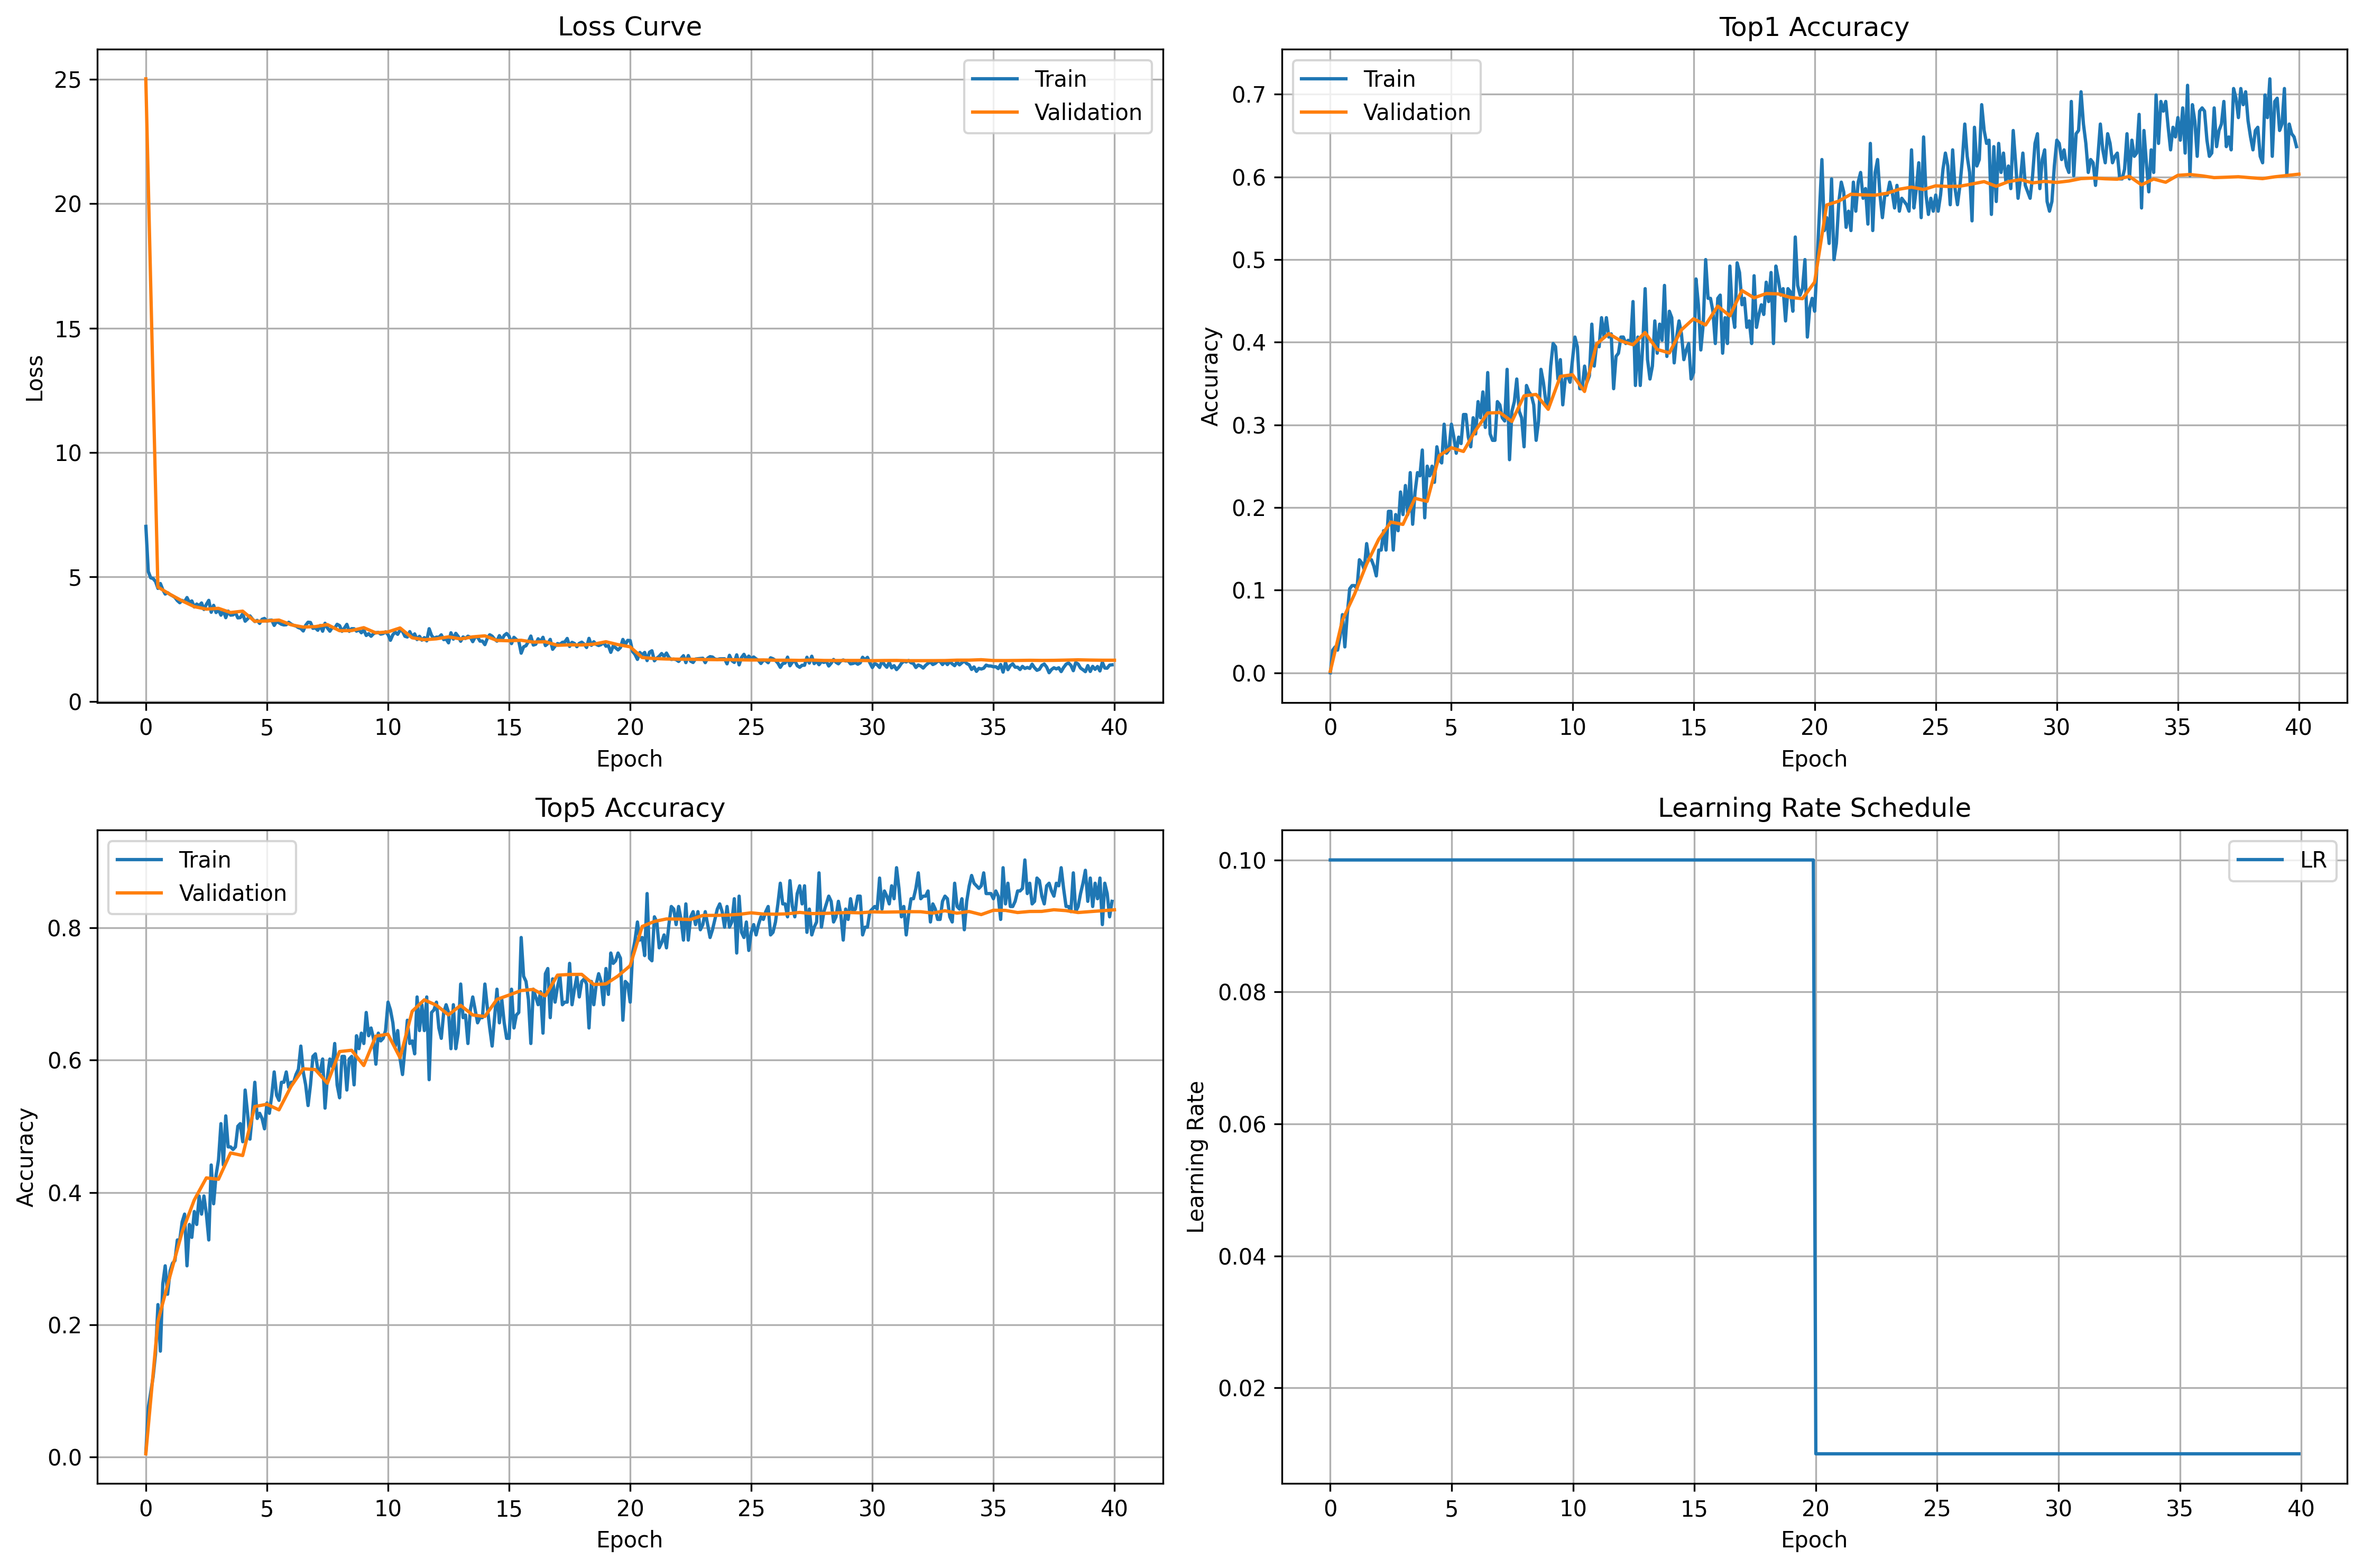
\includegraphics[width=0.9\linewidth]{cornet-s.png}
	\caption{CORnet-S训练数据变化图}
	\label{f.szxt}
\end{figure}

如图\ref{f.szxt}所示,在训练40个epoch后,模型达到其在验证集上的最佳表现。验证结果显示,模型的Top-1准确率为60.34\%,Top-5准确率为82.70\%,对应的交叉熵损失为1.6567。与此同时,模型在训练集上的Top-1准确率为63.67\%,Top-5准确率为83.98\%,训练损失为1.4718。验证集与训练集的准确率差距较小,表明模型在当前配置下未出现明显的过拟合现象,训练过程较为稳定。

\subsection{与原始论文结果对比}

原始的CORnet-S模型由Kubilius等人于2019年在NeurIPS会议中提出,其在ImageNet数据集上的Top-1准确率为74.4\%\cite{kubilius2019brain},在维持较小参数量的前提下,表现出接近ResNet-50的分类性能。同时,该模型在Brain-Score框架下的IT区神经预测得分也很高,被视为在准确率与类脑性之间达到较好平衡的代表性架构。

本文在Tiny-ImageNet-200数据集上复现了该类脑视觉模型,并使用标准训练配置进行训练与评估,最终在验证集上获得60.34\%的Top-1准确率和82.70\%的Top-5准确率。尽管该结果无法直接与原论文的ImageNet实验对齐,但在样本数量较少、图像尺寸较低的前提下,模型依然展现出稳定的识别能力,说明其结构在小样本多类别任务中同样具有较强适应性。

\begin{table}[htb]
	\centering
	\caption{CORnet-S准确率对比表}
	\label{tab:CORnet-S}
	\begin{tabular}{lllll}
		\hline
		       & 原始CORnet-S & 本文复现的CORnet-S \\
		\hline
		TOP1准确率 & 74.4\% & 60.34\%   \\
		TOP5准确率 & — & 82.70\%    \\
		\hline
	\end{tabular}
\end{table}

需要指出的是,Tiny-ImageNet的难度相较于完整的ImageNet仍有显著差异,类别缩减和图像简化可能会使模型更容易收敛。因此本实验的结果更多用于结构复现与改进对照,不可与完整ImageNet上的结果直接类比。但整体表现仍验证了CORnet-S模型在轻量级视觉任务中的有效性,也为后续结构优化与注意力机制集成提供了可靠的基线。

\section{基线可视化分析}

\subsection{中间激活图可视化分析}

为分析模型在各视觉皮层模拟层级的特征提取情况,本文使用forward hook方法提取了CORnet-S模型各层的中间激活图,并对典型通道的响应特征进行了可视化。

\begin{figure}[hbt]
	\centering
	
\includegraphics[width=0.6\linewidth]{car.jpg}
	\caption{激活图原图像}
	\label{f.car}
\end{figure}


在本实验中,选择CORnet-S模型的IT层作为可视化目标层,对验证集中典型图像样本进行激活响应分析。图\ref{f.cornet_s_jihuo}的(d)展示了该模型在IT层的六个典型通道的激活结果。

\begin{figure}[!htb]
	\centering
	\begin{subfigure}[t]{0.8\linewidth}
		\captionsetup{justification=centering}
		\begin{minipage}[b]{1\linewidth}
			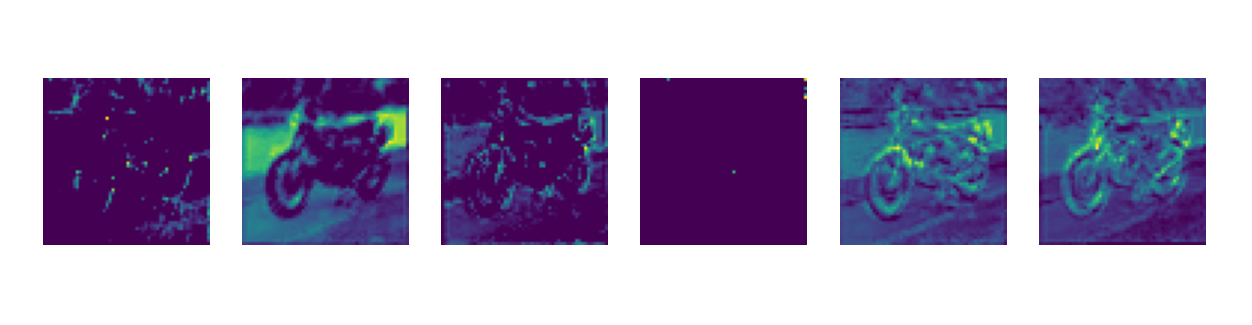
\includegraphics[width=1\linewidth]{V1_s_activations.png}
			\caption{V1层激活图}
		\end{minipage}
	\end{subfigure}\\
	\begin{subfigure}[t]{0.8\linewidth}
		\captionsetup{justification=centering}
		\begin{minipage}[b]{1\linewidth}
			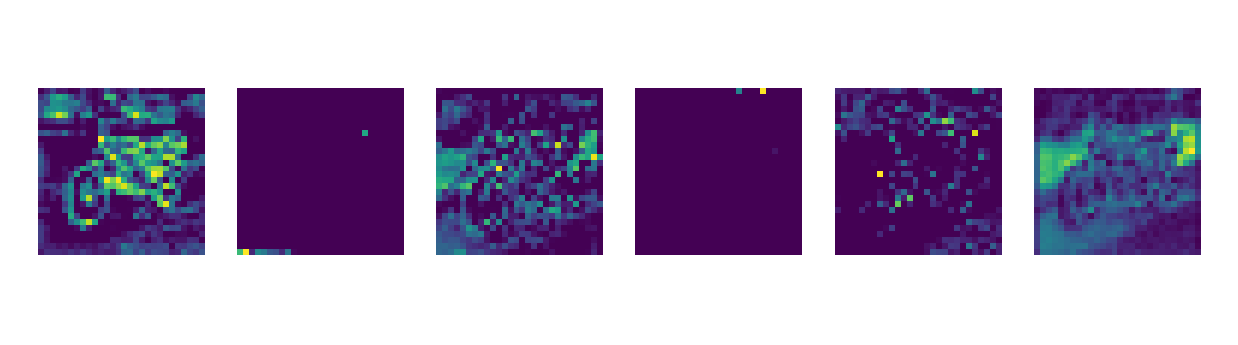
\includegraphics[width=1\linewidth]{V2_s_activations.png}
			\caption{V2层激活图}
		\end{minipage}
	\end{subfigure}\\
	\begin{subfigure}[t]{0.8\linewidth}
		\captionsetup{justification=centering}
		\begin{minipage}[b]{1\linewidth}
			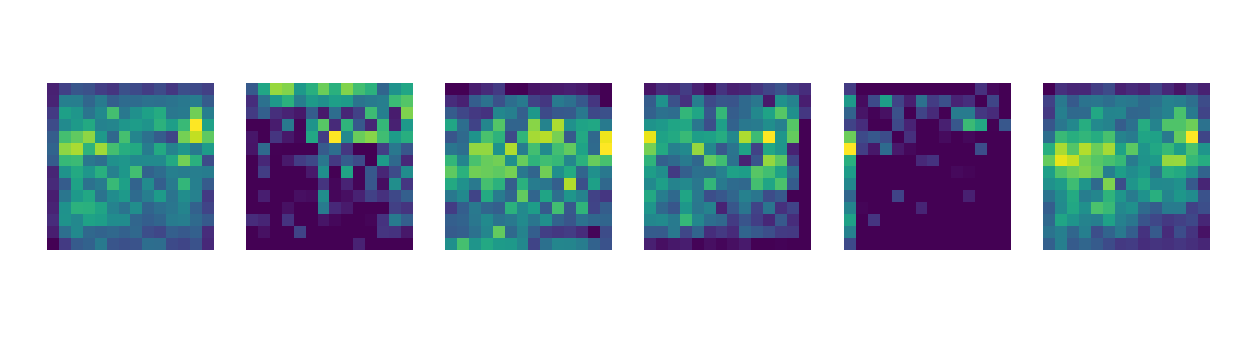
\includegraphics[width=1\linewidth]{V4_s_activations.png}
			\caption{V4层激活图}
		\end{minipage}
	\end{subfigure}\\
	\begin{subfigure}[t]{0.8\linewidth}
		\captionsetup{justification=centering}
		\begin{minipage}[b]{1\linewidth}
			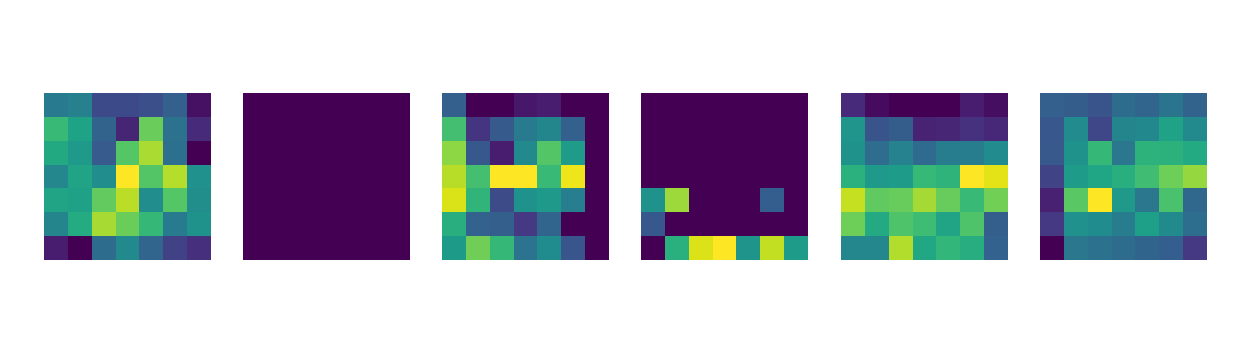
\includegraphics[width=1\linewidth]{IT_s_activations.png}
			\caption{IT层激活图}
		\end{minipage}
	\end{subfigure}
	\caption{CORnet-S模型各层激活图}
	\label{f.cornet_s_jihuo}
\end{figure}

观察图像可见,模型在多个通道中对图像主体区域(如摩托车轮廓、前轮等)产生了高响应,说明IT层能够聚焦于具有显著判别力的高阶语义特征。此外,部分通道对图像边缘或背景响应较弱,进一步印证该层在完成判别任务时具备一定的空间注意能力。

\subsection{关键区域关注能力探讨}

为进一步分析CORnet-S模型在不同层级的感知能力,图\ref{f.cornet_s_jihuo}的(a)至图\ref{f.cornet_s_jihuo}的(c)分别展示了模型在V1、V2和V4层的激活热力图。

从图\ref{f.cornet_s_jihuo}的(a)V1层可见,激活图主要集中在边缘与纹理区域,这表现出V1层为对图像整体结构的低级响应,体现了模型底层的感知特性。图\ref{f.cornet_s_jihuo}的(b)V2层中,响应区域虽仍零散,但开始聚焦于目标内部轮廓区域,初步展现出类别相关的空间感知。图\ref{f.cornet_s_jihuo}的(c)V4层显示出更集中的激活分布,尤其在图像的中部主体区域有明显增强,说明模型已完成对部分中层语义信息的整合。

尽管整体趋势符合生物视觉系统的层级响应特征,但部分激活图仍存在注意力漂移现象,如V1层的通道2与V2层的通道六对背景产生了强响应。这可能反映出当前模型在缺乏显式注意机制的条件下,其选择性聚焦能力存在一定的偏移,尤其在目标边界模糊、遮挡或图像背景复杂的场景下。

综上所述,激活图可视化结果表明,CORnet-S模型具有基本的空间关注能力和层级特征提取结构,但在判别区域的集中性与鲁棒性方面仍有改进空间。后续章节将尝试引入通道注意力机制,进一步优化模型对关键区域的响应特性。

